\noindent Se tienen dos láminas metálicas $a$ y $b$ de ancho despreciable y con carga uniformemente distribuida $Q$ y $-Q$, respectivamente. Cada lámina tiene un área $A$ y un largo $L$, que es mucho mayor que la separación entre las láminas. Entre $a$ y $b$ se encuentra una placa conductora de ancho $d$ a una distancia $h$ de cada una de las placas, como se muestra en la Figura \ref{fig:fig_1}.

\begin{figure}[H]
    \centering
    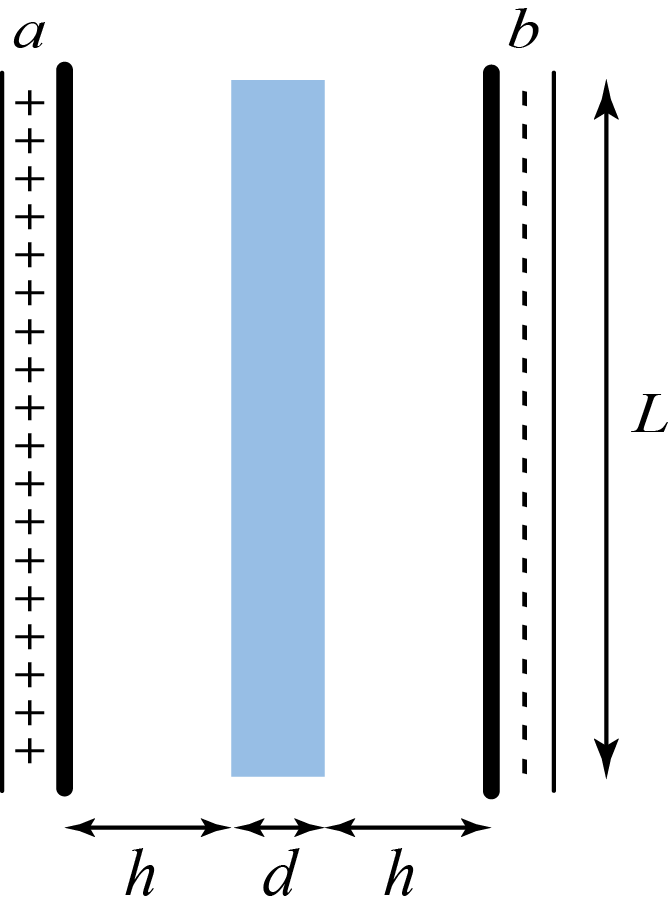
\includegraphics[height=5.5cm]{fig_1.png}
    \caption{Configuración Problema 1}
    \label{fig:fig_1}
\end{figure}

\begin{enumerate}[a)]
    \item Determine el campo eléctrico en todo el espacio entre las láminas.
    \item Calcule la diferencia de potencial entre las láminas.
    \item Determine la capacitancia del sistema. \\
    
    Ahora suponga que en lugar de una placa metálica hay un dieléctrico de permitividad $\epsilon$ que tiene las mismas dimensiones que la placa metálica. A partir de lo anterior:
    
    \item Determine el vector desplazamiento, campo eléctrico y vector polarización entre las láminas.
    \item Calcule la carga inducida en la superficie del material dieléctrico.
    \item Determine la capacitancia del sistema.
\end{enumerate}